To compare our \ourmethod to \psgd (data partition), \dsgd (sync barrier) and
\graphlab over speed of convergence and convergence quality we run
them over a collection of large real world dataset. To further demonstrate the
scalability of the approach we replicate and stack up real dataset to
artificially create datasets of terabytes scale. 

\subsection{Dataset}
\label{subsec:data}
We use three public datasets, \nytimes~\footnote{\url{http://archive.ics.uci.edu/ml/datasets/Bag+of+Words}},
\imagenet\footnote{\url{http://www.image-net.org/challenges/LSVRC/2010/download-public}}
and \twitter\footnote{\url{http://snap.stanford.edu/data/web-Stanford.html}} one each for
\lda, \dl and \mmsb respectively. \alex{this looks silly and is also
incomplete.  remove \{paragraphs\} and fill in with more details such as
gigabytes}
\paragraph{\nytimes} It is a collection of 300,000 Ny Times news articles that
contain 102,660 distinct words and 100,000,000 tokens (word occurrences) in the.
\paragraph{\imagenet} This dataset was originally used for large scale visual
recognition challenge in 2010~\cite{imagenet_cvpr09}. The set contains 1,261,406
images each with 1,000 features and has in total 389,080,708 non-zero pixels.
\paragraph{\twitter} This is a network of webpages from Stanford University's web-graph 
that stores directed edge between two webpages~\cite{Leskovec2008}. It consists of
2,312,497 edges distributed among 281,903 vertices (webpages). We make this graph denser 
by adding zero edges in the data explicitly. Any edge not present is simply ignored but
adding explicitly zero edges makes the model perform computation over it. We add as 
many edges as to make it fill 0.5\% of the total possible edges(0.5\% of 281903*281903=
796,756,340). We call this graph \swebgraph{1}.
\paragraph{\scaleblenytimes(\snytimes{N})} We replicate the documents in
\nytimes to create a \lda datasets that are in scales of hundreds of gigabytes. For example
\snytimes{4} is a datset that has each news article in \nytimes dataset
replicated 4 times. We create \snytimes{4}, \snytimes{16}, \snytimes{64} and
\snytimes{256} that have 1,200,000, 4,800,000, 19,200,000 and 76,800,000
documents with data sizes 6.08, 25.12, 103.4, and 421.42 GBs respectively.
Table~\ref{tab:dataset} shows the concise statistics of the dataset used in
all the experiments.
\paragraph{\scalebleimagenet(\simagenet{N})} Similar to scaling  \nytimes dataset
\imagenet data is replicated to test the scalability of the systems. We created
\simagenet{0.5},\simagenet{1.5}\simagenet{2}\ldots\simagenet{8} besides creating 
\simagenet{12} and \simagenet{16}. Table~\ref{tab:dataset} shows the different scaled 
datasets and their dimensions and sizes.
\paragraph{\scaleblewebgraph(\swebgraph{N})} Instead of increasing the dimension 
of the data i.e. number of vertices in the graph, we increase the edges. As discussed, 
we defined \swebgraph{1} as the graph that has 0.5\% of total possible edges. Similarly
\swebgraph{N} has $\frac{N}{2}$\% of total possible edges. The dimension of these 
datasets remain same as the original datatset, the increase happens in the number of 
edges (including explicit zero edges) as seen in table~\ref{tab:dataset}.  

% \begin{table}
% \centering
% \begin{tabular}{c|c|c|c|} %\hline
% Dataset  & Dimensions & Non-zeros & Size \\ \hline
% \nytimes  & 300,000$\times$102,660 & 100,000,000 &  1.49 Gbs \\ \hline
% \pubmed & 8,200,000$\times$141,043 &  730,000,000 & 11.19 Gbs \\ \hline
% \imagenet & 1,261,406$\times$1,000 & 389,080,708 & 5.06 Gbs \\ \hline
% \twitter & 41,652,230$\times$41,652,230 & 1,468,365,182 & 23.99 Gbs \\ \hline
% \snytimes{4} & 1,200,000$\times$102,660 & 400,000,000 &  6.08 Gbs \\ \hline
% \snytimes{4} & 4,800,000$\times$102,660 & 1,600,000,000 &  25.12 Gbs \\ \hline
% \snytimes{4} & 19,200,000$\times$102,660 & 6,400,000,000 &  103.4 Gbs \\ \hline
% \snytimes{4} & 76.800,000$\times$102,660 & 25,600,000,000 &  421.42 Gbs \\
% \hline
% \end{tabular}
% \end{table}


\begin{table}
\centering
\scalebox{0.95}{
\begin{tabular}{c|c|c|c|} %\hline
Dataset  & Dimensions & Nonzeros & Size(GB) \\ \hline
\nytimes  & $0.3*10^6\times$102,660 & $0.1*10^9$ &  1.49  \\ \hline
\imagenet & $1.26*10^6\times$1,000 & $0.39*10^9$ & 5.06  \\ \hline
\twitter & $41.6*10^6\times 41.6*10^6$ & $1.5*10^9$ & 23.99 \\ \hline
\snytimes{4} & $1,2*10^6\times$102,660 & $0.4*10^9$ &  6.08  \\ \hline
\snytimes{16} & $4.8*10^6\times$102,660 & $1.6*10^9$ &  25.12  \\ \hline
\snytimes{64} & $19.2*10^6\times$102,660 & $6.4*10^9$ &  103.4  \\ \hline
\snytimes{256} & $76.8*10^6\times$102,660 & $25.6*10^9$ &  421.42  \\ \hline
\hline
\end{tabular}
}
\caption{Dimension, size and nonzero statistics for different datasets. The
exact figures are rounded off for simplicity. Size is the file size in
gigabytes. The biggest dataset (\snytimes{256}) is of size approximately 0.5
terabytes.}
\label{tab:dataset}
\end{table}


\subsection{\graphlab based solver}
We modify \graphlab's collaborative filtering toolkit to add the constraints
defined in equation~\ref{eqn:constraints} \abhi{put in the constraints
equation}, Section~\ref{sec:applications}. We modify \sgd based learner of the toolkit as
it is eaisly pralleizable in the data space\abhi{Do we need to justify why we
use SGD based solver for graphlab?}.
We use its public APIs ( \textit{transform\_vertices(), periodic aggregator} and
\\\textit{map\_reduce\_vertices()}) to put normalization constraints. We take
the simplest and most efficient way of normalizing accross vertices. A periodic
aggregator is called after every fixed interval to compute the normalization
factor using \textit{map\_reduce\_vertices()} after which
we apply the computed factor to each vertex using \textit{transform\_vertices()}.


\begin{figure}
\centering
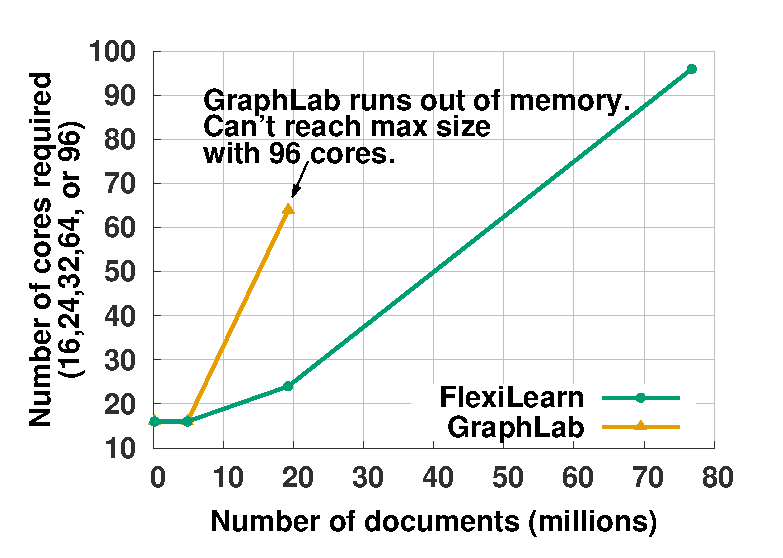
\includegraphics[width=0.46\textwidth]{fig2/lda_machines_failing.eps} 
\caption{The minimum number of machines needed vs the data size. We can see that \ourmethod 
is economic compared to graphlab for a given data size}
\label{fig:ldaMachinesNeeded}
\end{figure}



\begin{figure*}[t]
\centering
\begin{tabular}{|c|c|c|c|}
\hline
\multicolumn{4}{|c|}{\bf Topic Modeling} \\
\hline
Convergence Plots & \# of Topics & \# of Processors & \# of Docs \\
\hline
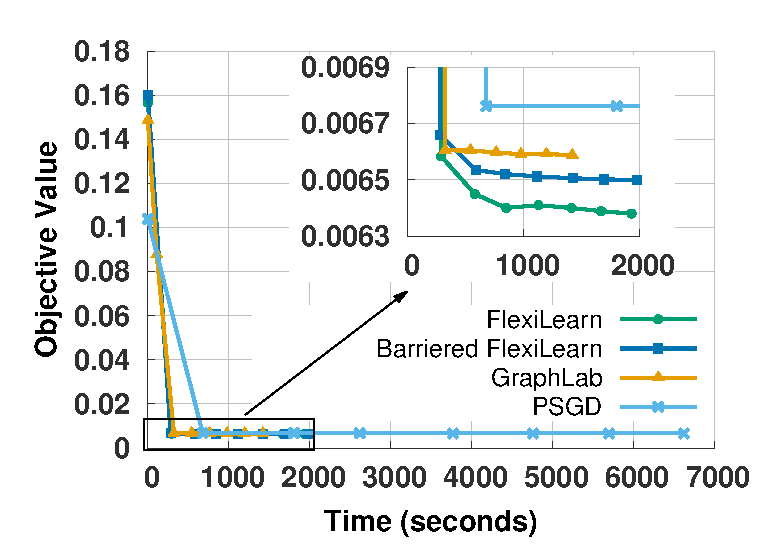
\includegraphics[width=0.23\textwidth]{fig2/lda_convergence.eps} &  
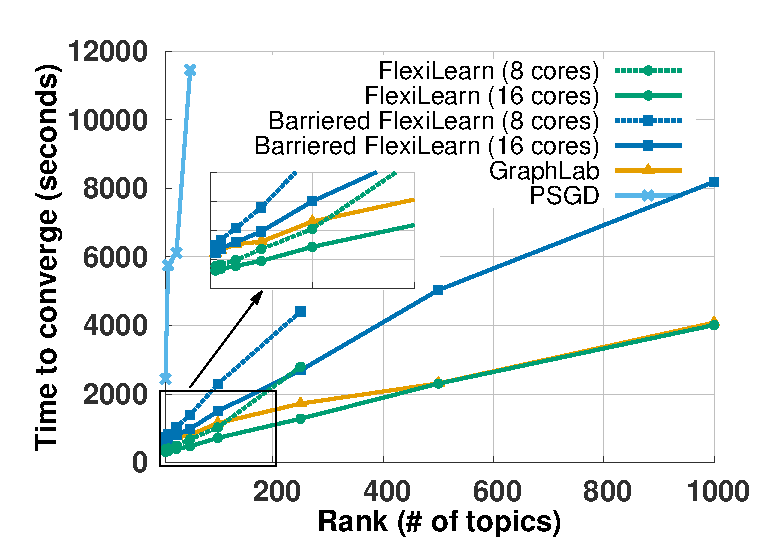
\includegraphics[width=0.23\textwidth]{fig2/lda_rankv3.eps} & 
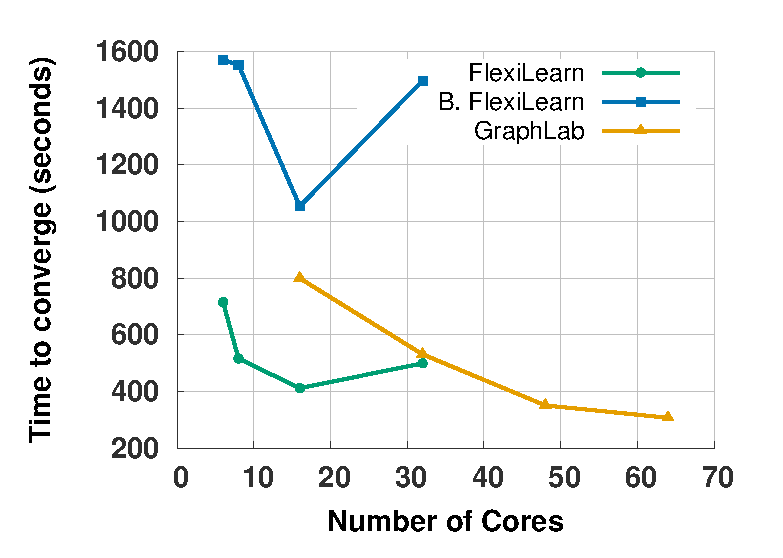
\includegraphics[width=0.23\textwidth]{fig2/lda_machines.eps} &
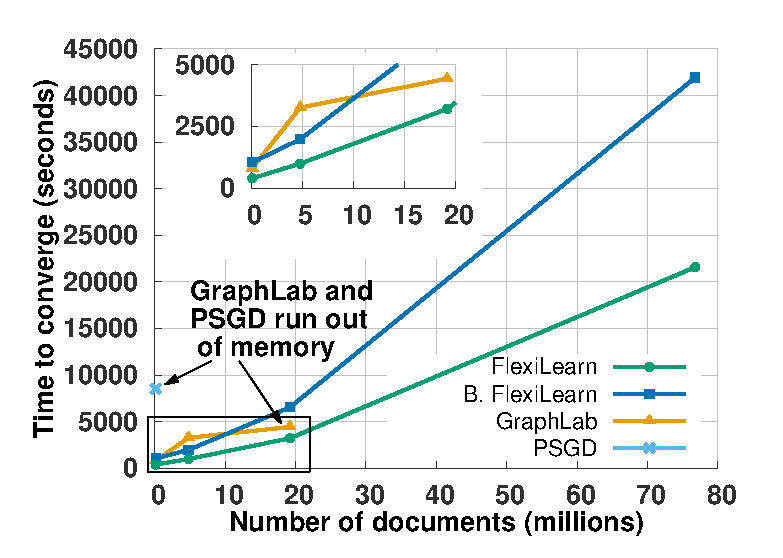
\includegraphics[width=0.23\textwidth]{fig2/lda_datasize.eps} \\
\hline
\multicolumn{4}{|c|}{\bf Dictionary Learning} \\
\hline
Convergence Plots & \# of Dictionary Bases & \# of Processors & \# of Images \\
\hline
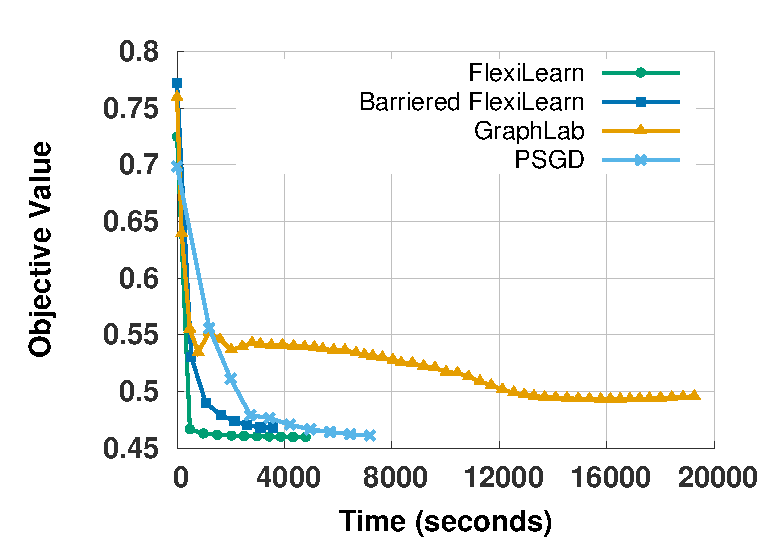
\includegraphics[width=0.23\textwidth]{fig2/dict_convergence.eps}& 
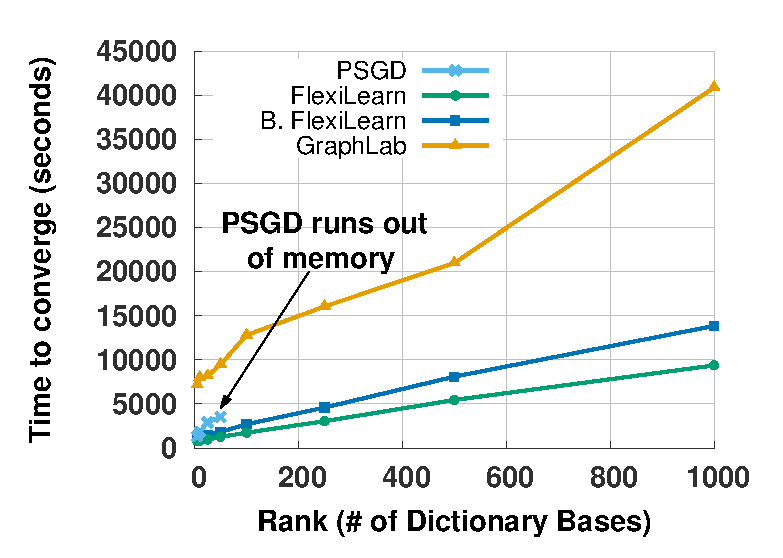
\includegraphics[width=0.23\textwidth]{fig2/dict_rank.eps} & 
TODO &
%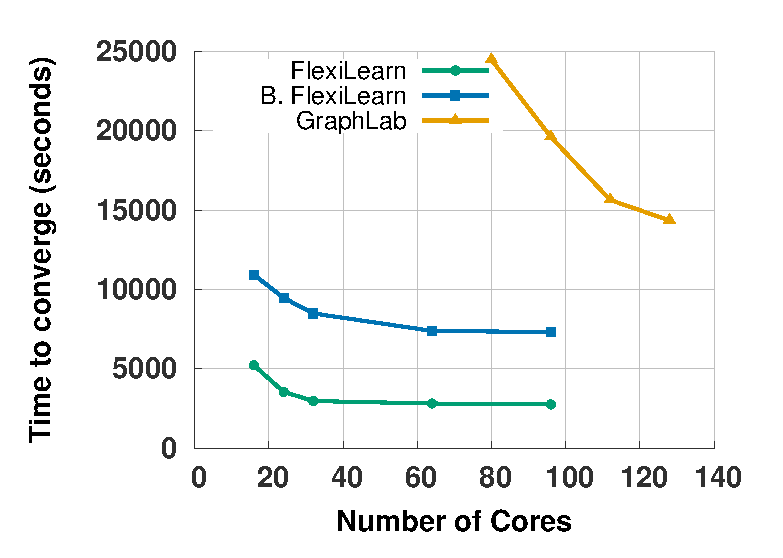
\includegraphics[width=0.23\textwidth]{fig2/dict_machines.eps} &
\includegraphics[width=0.23\textwidth]{fig2/dict_datasize.eps} \\
\hline
\multicolumn{4}{|c|}{\bf Mixed Membership Network Decomposition} \\
\hline
Convergence Plots & \# of Network Roles & \# of Processors & \# of Network Nodes \\
\hline
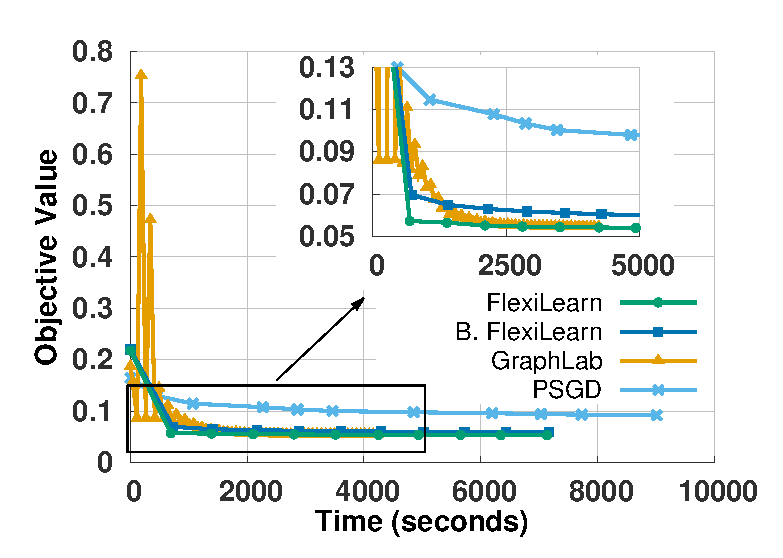
\includegraphics[width=0.23\textwidth]{fig2/mmsb_convergence.eps} &
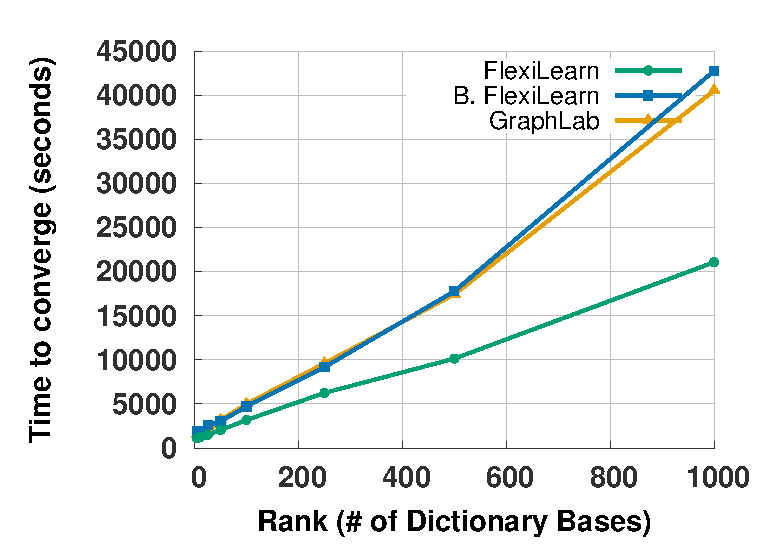
\includegraphics[width=0.23\textwidth]{fig2/mmsb_rank.eps} & 
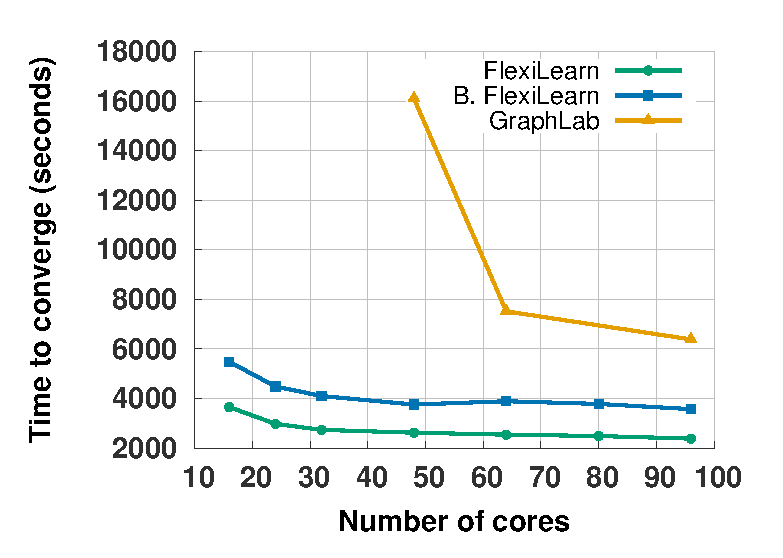
\includegraphics[width=0.23\textwidth]{fig2/mmsb_machines.eps} &
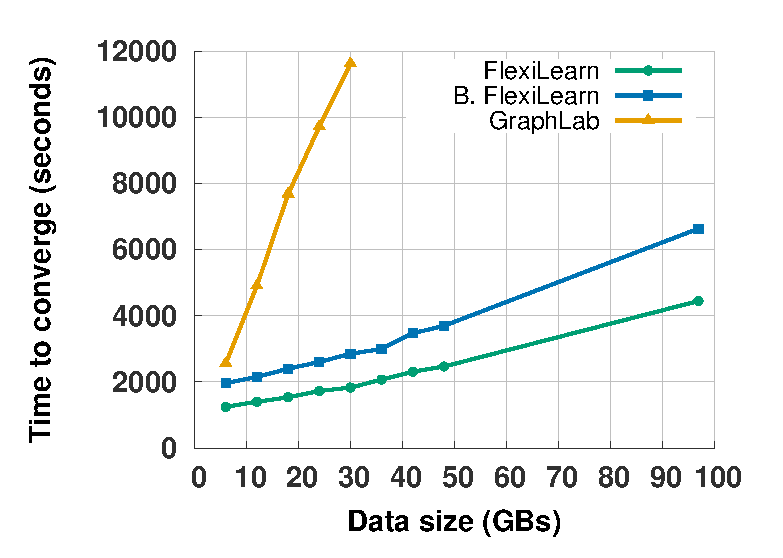
\includegraphics[width=0.23\textwidth]{fig2/mmsb_datasize.eps} \\
\hline
\end{tabular}
\caption{\small Convergence (Left) and scalability (in rank, processor cores and data size)
of all methods, on topic modeling, dictionary learning and mixed-membership network decomposition.
The convergence plot reveals the solution trajectory of each method, revealing pathological behavior such as oscillation.
The scalability plots show how each method fares as the problem rank, number of processor cores, and data
size is increased.}
\label{fig:results}
\end{figure*}

\subsection{Hardware Specifics} The Hadoop cluster used has 
2x Intel Xeon E5440@ 2.83GHz (8 cores per machine) machines each with 16GB RAM and 10Gbit
Ethernet. All three Hadoop based methods  (\ourmethod, \dsgd and \psgd) run on this cluster.
\graphlab is run on a different cluster as the Hadoop cluster didn't support MPI. The 
\graphlab cluster consists 2x Intel Xeon E5-2450 @2.1-2.9GHz (16 cores per machine)  with
128GB RAM and 10Gbit Ethernet. Thus \graphlab experimental setup has more memory but slightly 
slower machines.

\abhi{note down which dimensions (dimensions, rank, machines, density) are fixed to what 
for which experiments}
